%%%
% set up document type
%%%
\documentclass[12pt]{article}

%%%
% declare all packages
%%%
\usepackage[left=25mm, top=20mm, right=25mm, bottom=30mm,nohead,nofoot]{geometry} 

\usepackage[T2A]{fontenc}
\usepackage[utf8]{inputenc}
\usepackage[english, russian]{babel}

\usepackage{graphics, graphicx}

\usepackage{url}
\usepackage{hyperref}

\usepackage{amssymb,latexsym} 
\usepackage{MnSymbol}
\usepackage{mathrsfs}

\usepackage[nottoc,numbib]{tocbibind}
\usepackage{float}
\usepackage{listings}
\usepackage{multirow}
\usepackage{hhline}
\usepackage{delarray}

\usepackage{color,colortbl}

\usepackage{pdfpages}
\usepackage{csvsimple}

% \usepackage{verbatim}
%%%
% document settings
%%%
\setcounter{tocdepth}{4}
\graphicspath{ {./pic/} }

\renewcommand{\listoffigures}{\begingroup  % add number to list of graphics
\tocsection
\tocfile{\listfigurename}{lof}
\endgroup}
\renewcommand{\listoftables}{\begingroup  % add number to list of tables
\tocsection
\tocfile{\listtablename}{lot}
\endgroup}

%******************************************************************
%******************************************************************
\begin{document}

\begin{titlepage}
	\center
		Санкт-Петербургский Политехнический университет Петра Великого\\
		Институт прикладной математики и механики
		\\ \textbf{Высшая школа прикладной математики и вычислительной физики}

	\vfill ~
	\textbf{ \large Отчёт по научно-исследовательской работе } \\
    \large на тему: \\
	\large Визуализатор данных и ответов в вычислительной геометрии \\
	\large по направлению 01.04.02 `Прикладная математика и информатика` \\
	\large (профиль 01.04.02\_02 Математические методы анализа и визуализации данных) \\
	\vfill ~
	
    \begin{flushright}
    Cтудент группы 3640102/00201 \underline{\hspace{3cm}} Н.В.Лансков \linebreak[2]
    Cтудент группы 3640102/00201 \underline{\hspace{3cm}} М.А.Нахатович \linebreak[2]
	Оценка научного руководителя: \underline{\hspace{1cm}}\hspace{0.1cm} \underline{\hspace{3cm}} С.Э.Володарский\\  
    \end{flushright}

    
    
\vfill

{\large}Санкт-Петербург
\\ 2021 г
\end{titlepage}

%%%
% Table of conetnts 
%%%

\tableofcontents
\pagebreak
% \listoftables
% \newpage

\section{Введение}

Для решения задач вычислительной геометрии разрабатываются специальные программы. Такие программы получают данные и возвращают результаты в виде текстовых файлов. Глядя на столбцы чисел, бывает трудно понять, корректны ли входные данные и верно ли решение, которое выдала программа.
Проверки корректности входных и выходных данных могут быть реализованы в отдельной программе, 
но для каждой задачи нужна будет отдельная программа. В первоначальной отладке полезен инструмент, который отображает входные данные и решение. Целью данной работы является создание универсального инструмента для визуализации данных. Этот инструмент должен читать данные и ответы для широкого списка задач и отображать их в графическом виде.

\section{Постановка задачи}

Требуется создать универсальный текстовый формат для описания данных. Этот формат должен поддерживать входные и выходные данные задач из списка. Полный список задач приведён в приложении~\ref{apx}. Также требуется разработать приложение для визуализации данных, описанных с применением разработанного формата, на языке JavaScript. Приложение должно работать в браузере и поддерживать отрисовку больших объёмов данных. 
На вход программа получает текстовый файл с данными, которые требуется отрисовать. Описание данных должно соответствовать разработанному формату.

\section{Анализ существующих решений}

Самым известным решением является программа \textbf{GeoGebra} \cite{b1}. 

GeoGebra — это бесплатная, кроссплатформенная динамическая математическая программа, включающая в себя геометрию, алгебру, таблицы, графы, статистику и арифметику, в одном пакете. 

Однако, для наших целей она не подходит, так как обладает следующими недостатками:

\begin{enumerate}
	\item Поддерживает описание объектов только в формате XML, который трудно читать
	\item Не поддерживает отрисовку большого числа объектов ($\sim$100000).
\end{enumerate}

Поэтому было решено разработать собственное решение для визуализации данных.

\section{Описание проделанной работы}

\subsection{Текстовый формат}

В основе формата для описания данных было решено использовать \textbf{JSON} формат. Данный выбор обусловлен следующими преимуществами \textbf{JSON}:
\begin{enumerate}
	\item Встроенная поддержка во многих языках программирования, стандарт для \textbf{JavaScript}
	\item Поддержка автоматической валидации при помощи \textbf{JSON Schema} \cite{b4}
	\item Легко читается людьми
\end{enumerate}

Формат имеет следующую единообразную структуру: 
\begin{itemize}
	\item Любой документ, поддерживающий разработанный формат, содержит два поля: объект \textbf{elements} и массив \textbf{visualizations}
	\item Внутри поля \textbf{elements} содержатся все объекты, которые нужны для визуализации данных. Значение каждого поля объекта \textbf{elements}  может быть как  непосредственно  объектом визуализации (многоугольник, отрезок, точка и т.д.), так и списком таких объектов. Списки могут быть вложенными. Объекты визуализации содержат поле \textbf{type} с указанием типа объекта, а также другие поля, специфичные для указанного типа объекта. Кроме того, объекты также могут быть представлены ссылкой на другой элемент данных, описанный внутри \textbf{elements}
	\item Массив \textbf{visualizations} содержит объекты-ссылки на объекты данных, указанные в \textbf{elements}, которые требуется отрисовать
\end{itemize}

Таким образом, данный формат легко расширить новыми типами объектов.

\subsection{Приложение}

Для визуализации данных было разработано приложение на языке JavaScript. В качестве метода отрисовки был использован WebGL renderer, подключённый посредством библиотеки Three.js \cite{b5}. Возможности быстрого 'зумирования' и 'перемещения сцены' реализованы при помощи библиотеки D3.js\cite{b6}. 

Приложение состоит из трёх основных элементов интерфейса: меню, в котором есть возможность загрузить новый файл с данными для визуализации, блок информации, в котором отображается информация об отрисованных объектах, и непосредственно полотно для отрисовки графических данных. 

Также, приложение вычисляет некоторые простейшие метрики объектов, такие как, например, площадь и периметр многоугольников, для упрощения анализа результатов визуализации.

\pagebreak

\section{Результаты}

В качестве демонстрации работы приложения ниже приведены результаты визуализации некоторых задач (Рис.~\ref{fig:1}, Рис.~\ref{fig:2}, Рис.~\ref{fig:3}).

Доступна демо-версия программы\cite{b2}, и исходный код находится в открытом доступе\cite{b3}. 

\begin{figure}[ht!]
	\centering
	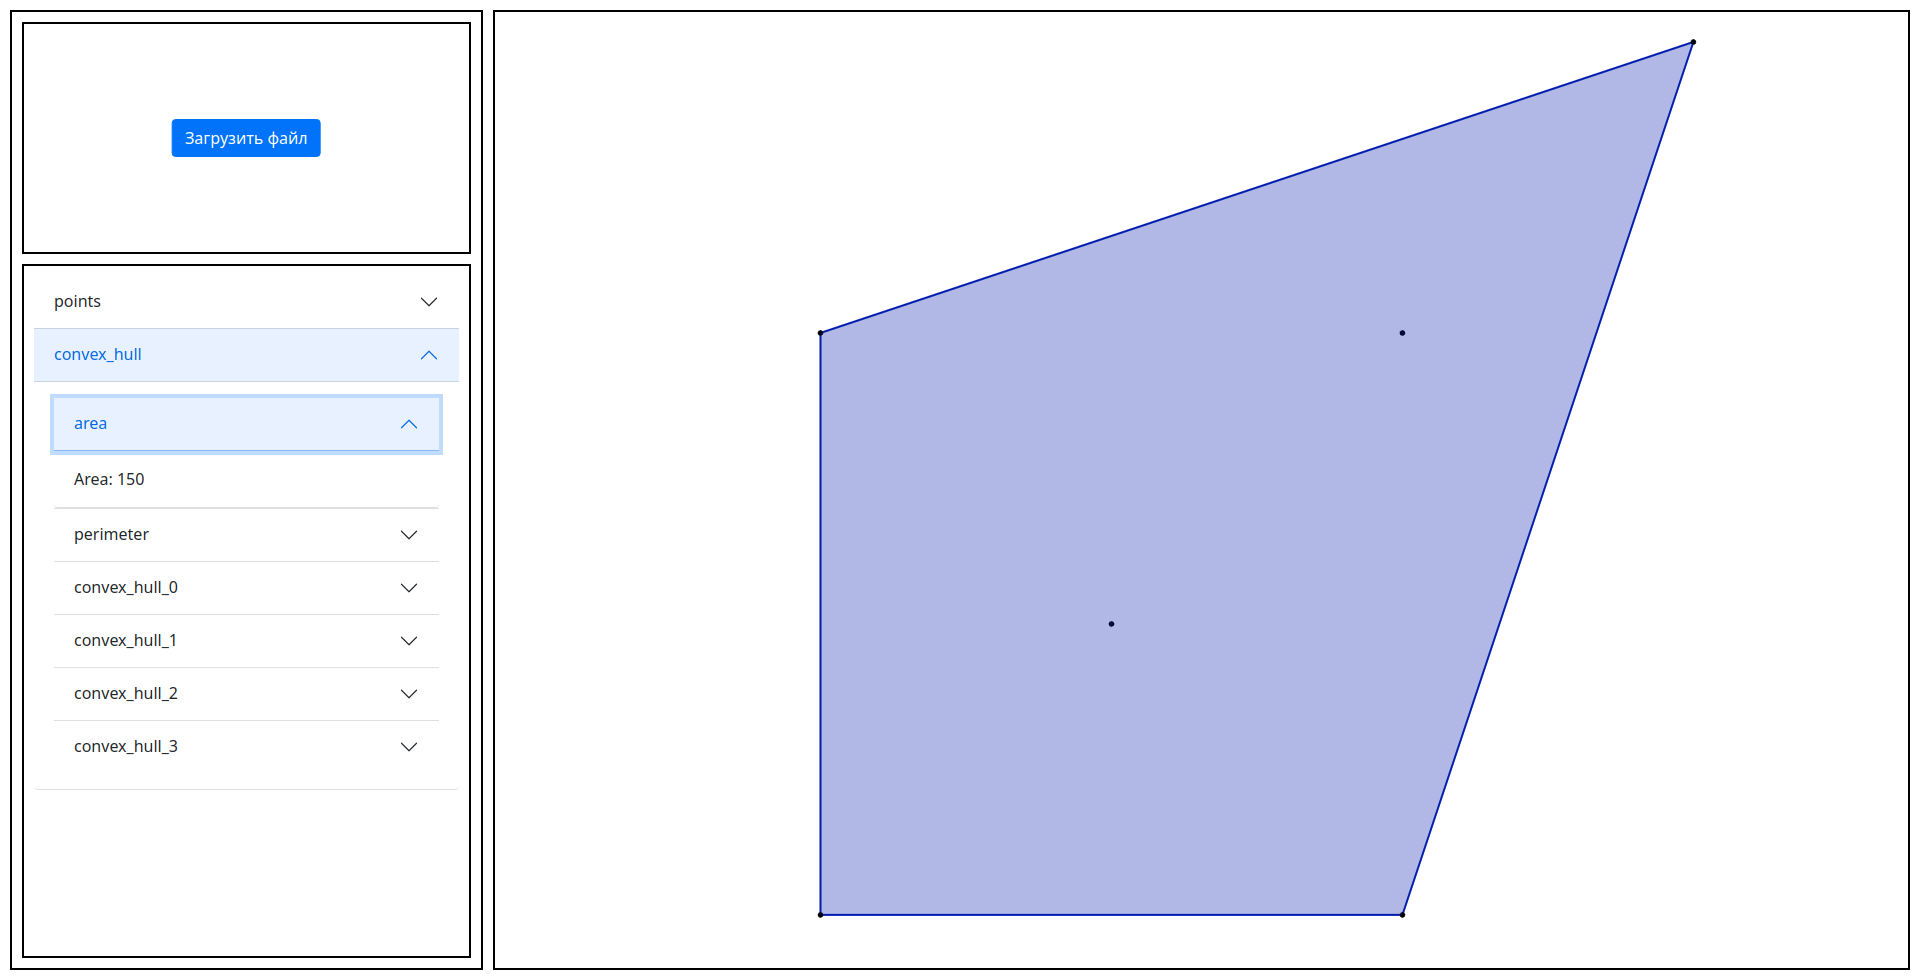
\includegraphics[width=.8\linewidth]{3.png}
	\caption{Построение выпуклой оболочки для множества точек}
	\label{fig:1}
\end{figure}

\begin{figure}[ht!]
	\centering
	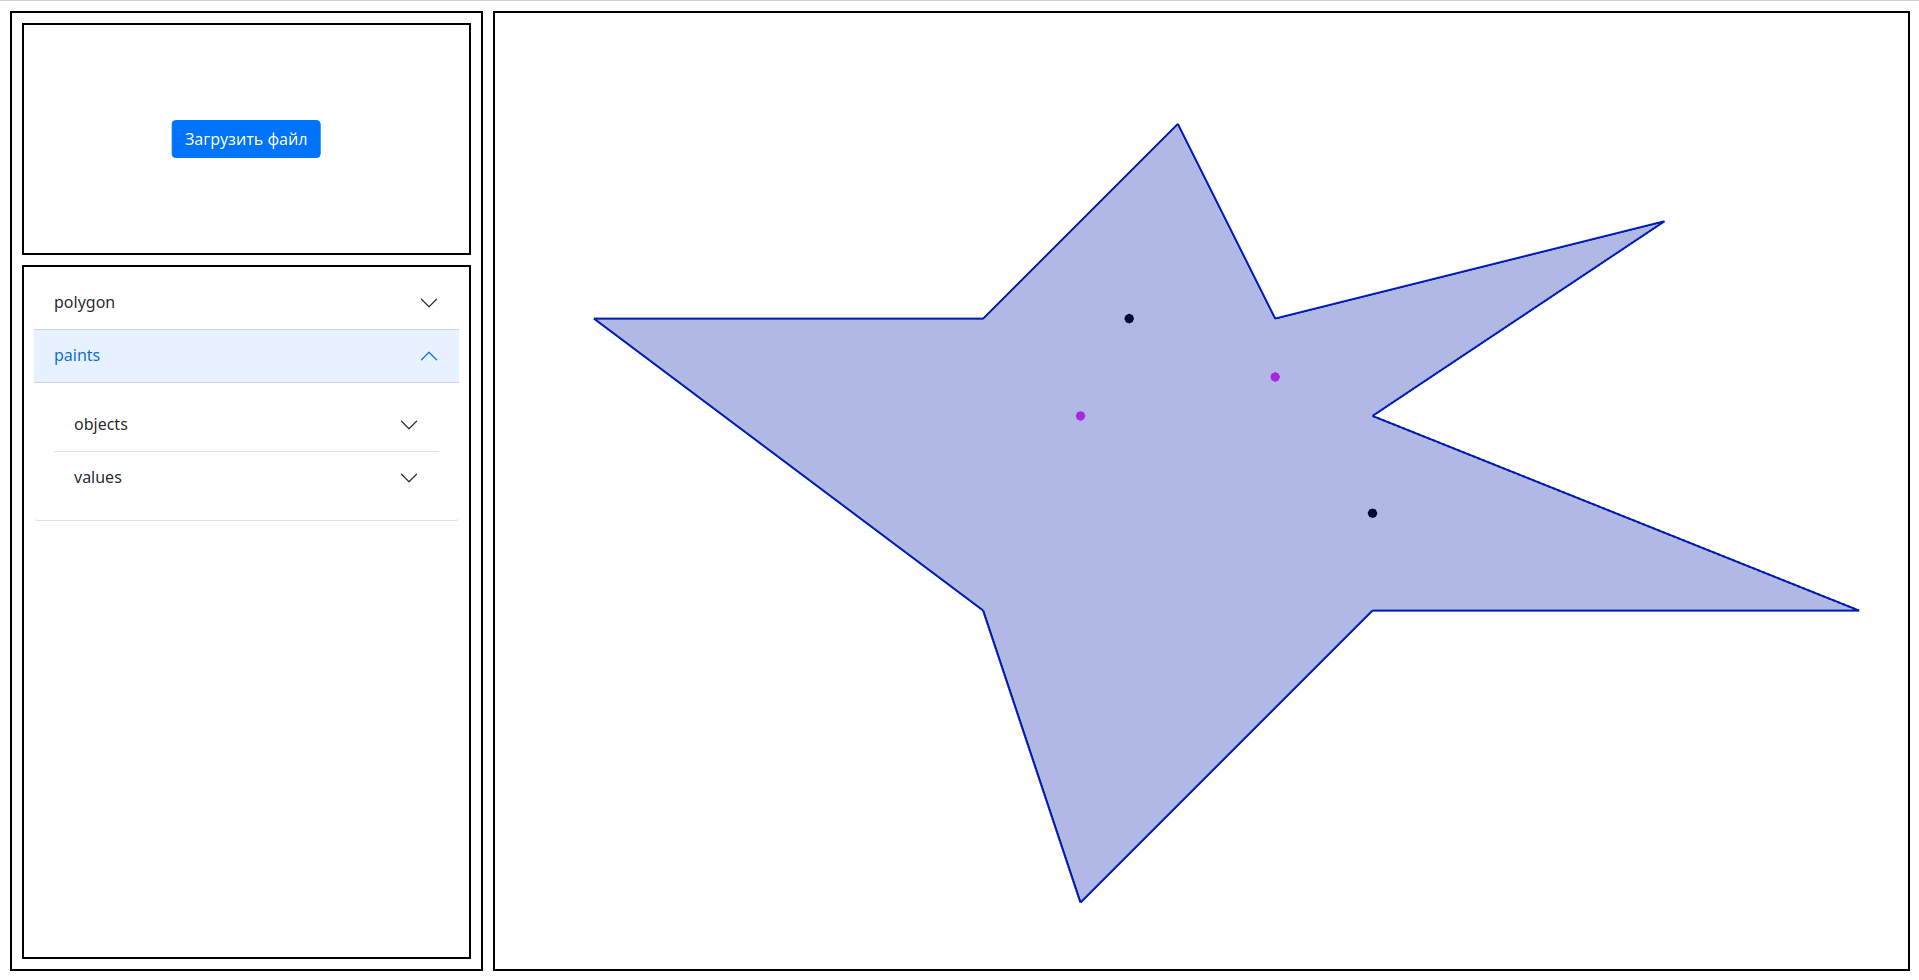
\includegraphics[width=.8\linewidth]{9.png}
	\caption{Проверка звёздности многоугольника для заданных точек}
	\label{fig:2}
\end{figure}

\begin{figure}[ht!]
	\centering
	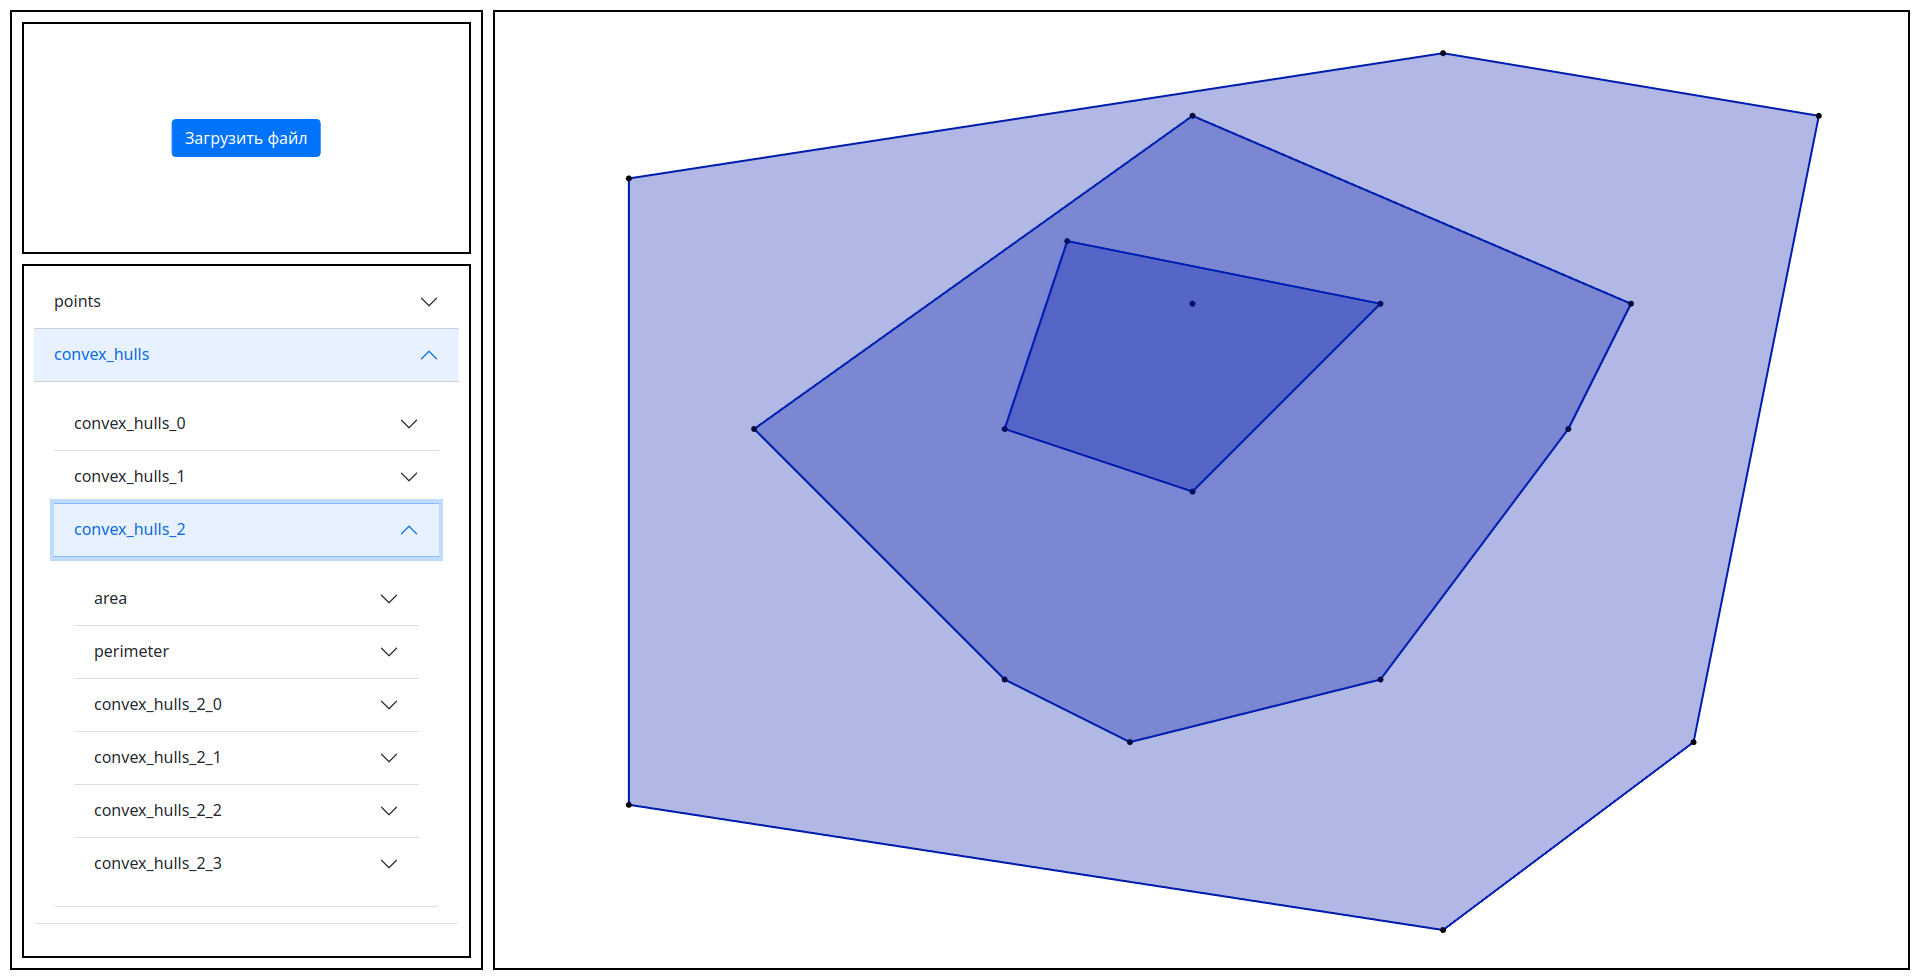
\includegraphics[width=.8\linewidth]{16.png}
	\caption{Задача о чистке лука}
	\label{fig:3}
\end{figure}

\pagebreak

\section{Описание дальнейшей работы} 

В дальнейшем требуется доработать графический  интерфейс программы, а также поддержать возможность отрисовки большего числа объектов.



\newpage

\listoffigures

\pagebreak

\begin{thebibliography}{5}


\bibitem{b1} GeoGebra, \url{https://geogebra.org}.
\bibitem{b2} Demo, \url{https://cg.leins275.xyz}.
\bibitem{b3} Code, \url{https://github.com/PrimatElite/cg-visualizer}
\bibitem{b4} JSON Schema, \url{https://json-schema.org/}
\bibitem{b5} Three.js, \url{https://threejs.org/}
\bibitem{b6} D3.js, \url{https://d3js.org/}


\end{thebibliography}

\newpage

\appendix
\section{Список задач}
\label{apx}

\begin{enumerate}
	\item Принадлежность точки многоугольнику
	\item Диаметр выпуклого многоугольника
	\item Выпуклая оболочка
	\item Минимальная опорная прямая для множества точек
	\item Ширина выпуклого многоугольника
	\item Пересечение выпуклых многоугольников
	\item Многоугольник на множестве вершин
	\item Проверка монотонности многоугольника (направления заданы)
	\item Проверка звёздности многоугольника (точки заданы)
	\item Пересечение полуплоскостей
	\item Проверка звёздности многоугольника (точка не задана)
	\item Пересечение ортогональных семейств отрезков
	\item Сумма Минковского двух выпуклых многоугольников
	\item Минимальный описанный прямоугольник для выпуклого многоугольника
	\item Диаграмма Вороного сторон выпуклого многоугольника
	\item Чистка лука
	\item Пересечение выпуклого многоугольника и прямой
	\item Триангуляция многоугольника (любой алгоритм)
	\item Экстремальная точка в выпуклом многоугольнике
	\item Число протыканий триангуляции выпуклого многоугольника
	\item Максимальный треугольник, вписанный в выпуклый многоугольник
	\item Минимальный диск для множества точек
	\item Диаграмма Вороного множества точек (любой алгоритм)
	\item Проверка триангуляции многоугольника
	\item Отыскание троек точек на одной прямой
		\pagebreak
	\item Максимальный круг, вписанный в выпуклый многоугольник
	\item Проверка простоты многоугольника
	\item Расстояние между выпуклыми многоугольниками
	\item Локализация точки в ППЛГ (любой метод)
	\item Ближайшая пара на плоскости
	\item Триангуляция Делоне (любой метод)
	\item Пересечение отрезков
	\item Пересечение ППЛГ
	\item Пересечение окружностей
	\item Восстановить множество точек по диаграмме Вороного

\end{enumerate}

\end{document}

